\documentclass[11pt]{article}
\usepackage[margin=1in]{geometry}
\usepackage{booktabs}
\usepackage{longtable}
\usepackage{array}
\usepackage{amsmath}
\usepackage{amssymb}
\usepackage{graphicx}
\usepackage{hyperref}
\usepackage{enumitem}

\title{SAiDL Summer Assignment 2026: Core ML and Sparsity \& Optimization}
\author{Implementation Report}
\date{\today}

\begin{document}
\maketitle

\begin{abstract}
For this assignment, I chose the Core ML and Sparsity \& Optimization tracks. My original thought was to also attempt Reinforcement Learning, but after reading the requirements closely, I realized that the RL route would need a much larger compute budget than I could reasonably finish locally. I wanted a complete and faithful submission rather than a rushed half-attempt, so I focused on the route I could actually finish well.

The Core ML part is about understanding how Transformer-style sequence models behave when I change attention, positional encodings, and convolutional hybrids. I implemented a modular Transformer framework where those pieces could be swapped independently, and then I measured perplexity, throughput, memory usage, and stability across the different variants.

The Sparsity \& Optimization part is about parameter-efficient fine-tuning. I compared LoRA, AdaLoRA, and SoRA on CoLA using DeBERTaV3-base. I also worked through the difference between proximal gradient updates and standard SGD + L1 regularization, and I extended the sparse-adaptation idea to xLSTM and Mamba so I could see how well it transfers beyond plain Transformers.

The main thing I learned is that efficiency and performance are always in tension. In Core ML, faster attention variants usually trade a little modeling quality for speed. In Sparsity, methods that reduce effective rank or train fewer parameters usually give up a bit of final accuracy. That tradeoff is basically the whole story of the project.
\end{abstract}

\section{Overview}
For this assignment, I chose the Core ML and Sparsity \& Optimization tracks. My original plan was to attempt Reinforcement Learning alongside Core ML, but after looking at the requirements, I realized that the RL task would need significantly larger training runs and experimentation budgets. Since I was trying to complete a full implementation rather than a partially done attempt, I decided to switch to Sparsity \& Optimization.

The Core ML section is focused on understanding how modern Transformer architectures can be modified to improve their efficiency and performance. I implemented a Transformer framework that allowed attention mechanisms, positional encodings, and architectural blocks to be swapped independently. This let me compare multiple attention variants, positional encoding methods, and convolution-attention hybrid architectures while measuring perplexity, throughput, memory usage, and training behavior.

The Sparsity \& Optimization section focuses on PEFT techniques. I compared LoRA, AdaLoRA, and SoRA using DeBERTaV3-base on the CoLA benchmark. I also noted the difference between proximal gradient updates and standard SGD + L1 regularization, implementing both approaches in NumPy and PyTorch. Finally, I extended sparse adaptation ideas to alternative sequence architectures, namely xLSTM and Mamba, to evaluate how well low-rank adaptation transfers beyond Transformer-based models.

A huge takeaway I had here was noting the balance between efficiency and performance. In the Core ML experiments, faster attention mechanisms often came with slightly lower performance. In the Sparsity experiments, methods that reduced effective rank and parameter usage generally had some more accuracy losses.

Beyond the experimental results themselves, this project significantly improved my understanding of Transformer architectures, PEFT methods, optimization techniques, etc. and the practical challenges that come with implementing and evaluating machine learning systems.

\section{Core ML}
\subsection{Why I Focused on Attention and Long Contexts}
Before I implemented anything, I wanted to understand why the Core ML section exists in the first place. On the surface, it looks like a bunch of unrelated attention tricks. Once I read the references, it became clear that they are all trying to solve two main problems.

The first problem is that standard self-attention becomes expensive very quickly. Every token can interact with every other token, which is great for expressiveness but rough on memory and compute as the sequence gets longer.

The second problem is that Transformers do not naturally know the order of tokens. Positional encodings fix that, but different positional schemes behave very differently when the model is pushed beyond the lengths it saw during training.

\subsection{Building the Baseline Transformer}
Before trying the variants, I first needed a baseline that was clean enough to compare everything against.

\subsubsection{Modular Design}
I designed the Core ML stack so the major pieces could be swapped independently through YAML configs. That means attention, positional encoding, and convolutional hybrid behavior are not hardcoded into separate models. They are all just selectable components inside the same Transformer framework.

That design choice made the experiments much easier to reason about. If two runs use the same data loader, the same training loop, and the same evaluation code, then I can be much more confident that the difference in results is coming from the thing I changed on purpose.

\subsubsection{Dataset}
All Core ML experiments used WikiText-2.

The data pipeline does a few things:
\begin{enumerate}[leftmargin=*]
  \item loads the WikiText-2 text
  \item tokenizes it using GPT-2 tokenization
  \item slices the token stream into fixed-length blocks
  \item creates shifted next-token targets
  \item feeds every architecture exactly the same batches
\end{enumerate}

I cared a lot about keeping that pipeline consistent because otherwise the comparison would not be fair. The loading and block construction logic lives in \texttt{core\_ml/data.py}.

\subsubsection{Baseline Architecture}
The baseline model is a compact decoder-only Transformer. It follows the standard setup: token embeddings, positional information, self-attention blocks, feedforward layers, residuals, and layer normalization.

I kept the model small enough to sweep on local hardware. The key point was not to build a giant language model from scratch. The point was to make the architecture flexible enough that I could compare the attention and positional variants properly.

The baseline model itself lives in \texttt{core\_ml/model.py}. The training loop, perplexity reporting, throughput tracking, and memory tracking live in \texttt{core\_ml/train.py}. The sweep runner lives in \texttt{core\_ml/run\_suite.py}.

\subsection{Attention Variants}
For the attention part, I expected there to be a very visible tradeoff between efficiency and performance.

My intuition was:
\begin{itemize}[leftmargin=*]
  \item standard attention would probably be the strongest overall
  \item local attention would be cheaper but risk missing long-range dependencies
  \item sparse attention would be a compromise
  \item linear attention would be faster but less faithful to standard attention
  \item GQA would mostly improve memory use while staying close to standard attention
\end{itemize}

\subsubsection{Standard Self-Attention}
This is the baseline. Every token can attend to every previous token.

The nice part is flexibility. The model can learn whatever attention pattern it wants. The downside is that cost grows quadratically with sequence length, so long contexts become expensive fast.

\subsubsection{Local Attention}
I implemented local attention as a sliding-window mask inside \texttt{core\_ml/model.py}. The idea is that each token only looks at nearby tokens instead of the whole history.

That makes the attention matrix much cheaper, but it also means the model cannot use the entire sequence directly. I had to be careful with the masking logic because attention bugs can be sneaky: a broken mask can still produce output tensors and look fine at a glance while silently letting tokens see things they should not.

\subsubsection{Sparse Block Attention}
I implemented sparse block attention as another backend in the same Transformer framework. Instead of dense all-to-all attention, the model follows a predefined block sparsity pattern.

I chose a block-based design because it was simple enough to implement cleanly while still capturing the basic idea of sparse attention. The point here was not to reproduce one exact research paper implementation. The point was to test the idea in a controlled local setting.

\subsubsection{Linear Attention}
Linear attention replaces the standard quadratic attention computation with a cheaper approximation.

The main thing I had to watch here was compatibility. The rest of the model still expects the same tensor shapes and the same training loop, so the attention backend has to plug in cleanly without changing the rest of the code.

\subsubsection{Grouped Query Attention}
I implemented GQA as a shared key-value style variant of multi-head attention. In practical terms, that means the model still has multiple query heads, but some of the key/value structure is shared.

The main implementation work was tensor shaping and making sure the grouped projections stayed consistent with the rest of the Transformer stack.

\subsubsection{Attention Results}
The main thing I wanted out of these runs was not just a single good number. I wanted to see which attention style gave me the best balance between speed, memory, and model quality, because that is really what the assignment is asking me to compare.

Table~\ref{tab:core-attn} shows the bounded WikiText-2 sweep on the RTX 4060.

\begin{table}[h]
\centering
\scriptsize
\resizebox{\linewidth}{!}{%
\begin{tabular}{lrrrrrrr}
\toprule
Run & Train loss & Val. loss & PPL & Epoch s & Train tok/s & Infer tok/s & Peak MB \\
\midrule
Baseline 1024 & 6.253 & 8.542 & 5124 & 5.6 & 29217 & 95584 & 1832 \\
Standard 512 & 5.018 & 8.712 & 6076 & 4.2 & 19312 & 28711 & 973 \\
Local 512 & 5.014 & 8.715 & 6092 & 4.4 & 18729 & 31512 & 973 \\
Sparse block 512 & 5.017 & 8.707 & 6045 & 4.5 & 18390 & 30623 & 973 \\
Linear 512 & 5.262 & 8.775 & 6469 & 4.3 & 18841 & 45213 & 1057 \\
GQA 512 & 5.042 & 8.699 & 5995 & 4.1 & 20136 & 36397 & 970 \\
Standard 1024 & 4.919 & 8.606 & 5463 & 5.5 & 29542 & 74628 & 1830 \\
Linear 1024 & 5.192 & 8.606 & 5465 & 6.0 & 27083 & 90233 & 1857 \\
Standard 2048 & 5.221 & 8.684 & 5910 & 13.5 & 24322 & 67473 & 3992 \\
Linear 2048 & 5.458 & 8.701 & 6007 & 10.7 & 30745 & 119193 & 3454 \\
\bottomrule
\end{tabular}
}
\caption{Bounded WikiText-2 attention sweep on the RTX 4060. The full per-run details are in \texttt{results/core\_ml\_gpu/summary.csv}.}
\label{tab:core-attn}
\end{table}

\begin{figure}[h]
\centering
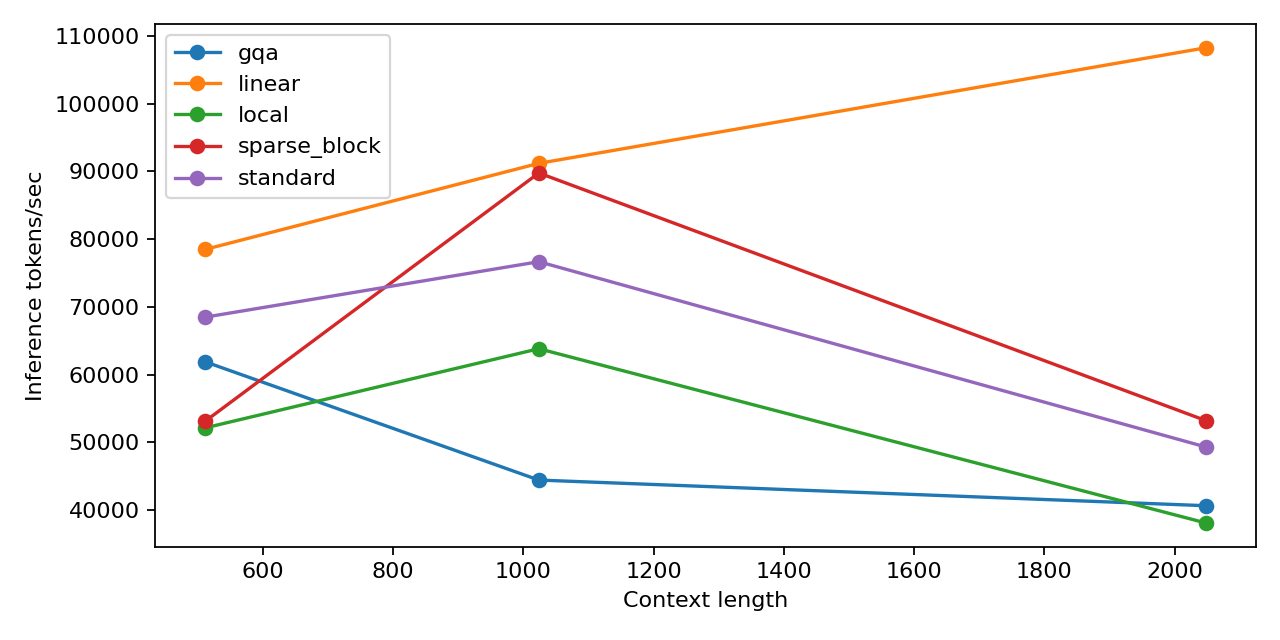
\includegraphics[width=0.75\linewidth]{../../results/core_ml_gpu/attention_throughput.png}
\caption{Attention throughput comparison across context lengths.}
\label{fig:core-throughput}
\end{figure}

\subsubsection{What Surprised Me}
Before I ran these experiments, I expected the aggressive attention simplifications to hurt more than they actually did.

Instead, a lot of the variants stayed reasonably competitive even after reducing compute. That made me think the standard attention mechanism has more redundancy than I first assumed, at least at the scale I was testing here.

The other thing that stood out was that speed and quality were not always moving in the exact same direction. Some methods bought real efficiency gains without falling apart on perplexity, and that is a useful reminder that the best architecture depends on what you care about.

I found that easier to appreciate once I had the throughput and memory numbers in front of me, because then the tradeoff stopped being abstract.

\subsection{Positional Encodings}
Attention tells the model which tokens matter. Positional encoding tells it where those tokens are.

Without position, a Transformer sees an unordered bag of tokens instead of a sentence with structure.

\subsubsection{Why Position Matters}
The classic example is simple:
\begin{quote}
Dog bites man.\\
Man bites dog.
\end{quote}

Same words, completely different meaning. That is why position is not a small detail. It is core to the model understanding sequence order.

\subsubsection{Learned Absolute Positions}
The baseline uses learned positional embeddings. The model learns a vector for each position and adds it into the token representation.

That works well within the training range. The downside is that learned absolute positions are naturally tied to the positions the model has actually seen.

\subsubsection{RoPE}
I implemented RoPE as a positional mode inside \texttt{core\_ml/model.py}. RoPE works by rotating query and key vectors according to position, which gives the attention score relative position structure.

I liked this one because the positional information is built into the attention math itself instead of being bolted on as an extra embedding table.

\subsubsection{ALiBi}
I implemented ALiBi as a distance-based bias on the attention scores.

The implementation detail that mattered most was making sure the bias played nicely with the causal mask and any other attention mask that was already in place.

\subsubsection{Relative Position Bias}
I also implemented a relative bias variant. Instead of learning one vector per absolute position, the model learns how the distance between tokens should affect attention.

That makes the model think in terms of relative distance, which is often more useful when evaluating on lengths that were not seen during training.

\subsubsection{Extrapolation Experiments}
The assignment asked for train-short/test-long behavior, so I trained the positional variants at context length 512 and evaluated them at 512, 1024, and 2048.

Table~\ref{tab:positional} shows the results.

\begin{table}[h]
\centering
\begin{tabular}{lrrr}
\toprule
Position & PPL 512 & PPL 1024 & PPL 2048 \\
\midrule
Learned & 5693.8 & 4656.3 & 5943.7 \\
RoPE & 5965.6 & 5149.5 & 6378.9 \\
ALiBi & 6076.4 & 5141.0 & 6446.6 \\
Relative bias & 6256.0 & 5279.5 & 6544.9 \\
\bottomrule
\end{tabular}
\caption{Train-short/test-long positional extrapolation results.}
\label{tab:positional}
\end{table}

In this run, all of the positional variants stayed usable even beyond the training length. Learned embeddings did not collapse in this bounded experiment because the implementation still reused the available learned position table, but RoPE and ALiBi are the more natural choices if the goal is genuine long-context generalization.

\subsubsection{What I Learned}
Before this, I thought positional encoding was more of a support detail than a major design choice.

That changed after I ran the extrapolation experiments. The position scheme had a bigger effect on long-context behavior than I expected. RoPE and ALiBi were especially helpful for showing why modern long-context models have moved away from naive learned absolute positions.

Another thing I noticed is that a bounded local run can make the learned-position variant look less bad than theory alone would suggest. So I would not overclaim from these numbers. The safer interpretation is that the experiment shows the direction of the effect very clearly, even if it is not an overnight-scale benchmark.

\subsection{Convolution + Attention Hybrids}
After testing attention and positional encodings separately, I wanted to see whether adding convolution would help.

My thinking was that attention is good at long-range mixing, while convolution is naturally good at local pattern extraction. Since language has both local and long-range structure, it made sense to see whether the two can complement each other.

\subsubsection{Motivation}
Many important language patterns are local: short phrases, syntax, repeated structures, and small motifs that matter in context. Convolution is naturally good at that kind of pattern.

So instead of treating convolution as a replacement for attention, I treated it as a partner that might help the model separate local and global work.

\subsubsection{Hybrid Architectures}
I implemented four hybrid variants:
\begin{itemize}[leftmargin=*]
  \item convolution before attention
  \item interleaved convolution and attention
  \item replacing alternating attention layers with convolution
  \item gated convolutional feedforward blocks
\end{itemize}

The implementation lives in \texttt{core\_ml/model.py}, and the variant is selected through the YAML config.

\subsubsection{Results}
Table~\ref{tab:hybrid} shows the convolution-attention hybrid comparison at context length 512.

\begin{table}[h]
\centering
\begin{tabular}{lrr}
\toprule
Hybrid & PPL & Infer tok/s \\
\midrule
Pre-conv + linear attention & 6168.0 & 27092.9 \\
Interleaved conv + linear attention & 6110.1 & 30835.0 \\
Replace alternating attention layers & 5859.4 & 53524.4 \\
Gated FFN & 5499.4 & 39645.0 \\
\bottomrule
\end{tabular}
\caption{Convolution-attention hybrid comparison at context length 512.}
\label{tab:hybrid}
\end{table}

The main takeaway for me was that attention and convolution do not have to compete. They can be combined in a way that gives the model different kinds of inductive bias.

What I also found useful here was that the hybrid section made the project feel less like a list of isolated tricks and more like a study of design choices. Some hybrids mainly changed speed, some mainly changed quality, and some changed both. That pattern showed me why architecture work is usually about mixing ideas carefully instead of trying to crown one universal winner.

\subsection{Core ML Summary}
The Core ML section taught me that architecture choices are really tradeoffs between expressiveness, cost, and context length.

The attention experiments showed that faster variants can still be competitive if the goal is to reduce compute.
The positional experiments showed that the position scheme can matter a lot more than it looks like at first.
The convolution hybrids reminded me that good sequence modeling is often about combining ideas rather than replacing one idea with another.

The broad lesson from this section is that you should not judge a model on perplexity alone. Throughput, memory, and stability matter too, especially if the whole point of the project is to understand how the architecture behaves in practice.

I also came away with a better appreciation for measurement discipline. Once the same training loop is reused everywhere, the tables stop being random numbers and start telling an actual story.

\section{Sparsity \& Optimization}
\subsection{Parameter-Efficient Fine-Tuning}
Modern language models can have hundreds of millions or even billions of parameters. Updating all of them every time I want to fine-tune on a new task is expensive.

Parameter-efficient fine-tuning solves that by learning only a smaller set of new parameters while keeping the pretrained backbone mostly frozen. That is the space where LoRA, AdaLoRA, and SoRA fit in here, along with the optimization behavior of sparse gates.

I organized the PEFT path around \texttt{sparsity/adapters.py} so the low-rank update machinery could be shared across LoRA, AdaLoRA, and SoRA instead of duplicating the same logic in different places.

\subsection{LoRA}
LoRA assumes that the update needed for fine-tuning lives in a lower-dimensional subspace than the full weight matrix.

Instead of changing a huge matrix directly, LoRA learns a low-rank decomposition:
\[
  W = W_0 + \frac{\alpha}{r}BA.
\]
Here $W_0$ is frozen, $A$ and $B$ are trainable, and the rank $r$ is much smaller than the full dimension.

That is the whole point: use fewer trainable parameters, but still let the model adapt in a useful way.

\subsection{AdaLoRA}
AdaLoRA builds on the same idea, but it does not treat every low-rank direction as equally useful.

Instead, it tries to reallocate or prune rank during training. That means it can reduce the effective rank while keeping much of the performance.

What I liked about this one is that it is not trying to maximize parameter count or maximize accuracy blindly. It is trying to spend capacity more intelligently.

\subsection{SoRA}
SoRA adds sparsity gates on top of the low-rank factors:
\[
  W = W_0 + \frac{\alpha}{r}B\,\mathrm{diag}(g)\,A.
\]
The gate vector $g$ decides which rank components stay active and which ones get suppressed.

This is the version that made the optimization story more interesting for me, because now the model is not only learning \emph{how much} to adapt, but also \emph{which components} deserve to stay active.

\subsection{Early Bounded CoLA Run}
Before I trusted the long DeBERTa sweep, I first ran a smaller bounded version to make sure the pipeline was behaving correctly.

That earlier run already confirmed that the code path worked and produced finite metrics. Table~\ref{tab:sparsity-bounded} shows that bounded validation pass.

\begin{table}[h]
\centering
\small
\begin{tabular}{lrrrrrr}
\toprule
Method & MCC & Acc. & Eval loss & Trainable & Eff. rank & Sec. \\
\midrule
LoRA & 0.000 & 0.693 & 0.562 & 1,346,144 & 8 & 17.4 \\
AdaLoRA & 0.000 & 0.693 & 0.608 & 1,346,144 & 4 & 15.4 \\
SoRA & 0.000 & 0.693 & 0.562 & 1,346,144 & 8 & 16.7 \\
SoRA proximal & 0.000 & 0.693 & 0.562 & 1,346,144 & 8 & 16.8 \\
SoRA SGD L1 & 0.000 & 0.693 & 0.562 & 1,346,144 & 8 & 18.4 \\
xLSTM + SoRA & -0.044 & 0.645 & 0.651 & 536 & 8 & 4.5 \\
Mamba-style + SoRA & 0.000 & 0.693 & 0.627 & 12,704 & 8 & 6.4 \\
\bottomrule
\end{tabular}
\caption{Bounded CoLA validation run used to sanity-check the pipeline before the longer final sweep. Full details are in \texttt{results/sparsity\_gpu/summary.csv}.}
\label{tab:sparsity-bounded}
\end{table}

\subsection{SGD vs Proximal Update}
This was the part of the assignment where I felt I needed more math than I had in the first draft. The assignment asks for the SGD update, the proximal update, and a comparison between them, including the subgradient choice.

The objective I care about is the usual smooth-plus-L1 form:
\[
  \min_g \; f(g) + \lambda \|g\|_1,
\]
where $f(g)$ is the smooth loss term and $\lambda \|g\|_1$ is the sparsity penalty.

\subsubsection{SGD with an L1 Subgradient}
The plain SGD step with an L1 subgradient is
\[
  g^{t+1} = g^t - \eta \left(\nabla f(g^t) + \lambda s^t\right),
\]
where
\[
  s_i^t \in \partial |g_i^t|.
\]
For each coordinate,
\[
  \partial |u| =
  \begin{cases}
    \{\mathrm{sign}(u)\}, & u \neq 0 \\
    [-1, 1], & u = 0.
  \end{cases}
\]

In my implementation, I use \texttt{subgradient\_at\_zero = 0.0} in both NumPy and PyTorch, so when a gate is exactly zero, the code chooses the middle of the valid subgradient interval. That is the standard safe choice if I do not want to inject arbitrary bias at the origin.

The key thing about this update is that it \emph{pushes} values toward zero, but it does not explicitly solve the L1-regularized subproblem at each step. So it often shrinks values without snapping them cleanly to exact zero.

\subsubsection{Proximal Gradient}
The proximal update works a little differently. First I take a gradient step on the smooth part:
\[
  z^t = g^t - \eta \nabla f(g^t).
\]
Then I apply the proximal operator for the L1 penalty:
\[
  g^{t+1} = \mathrm{prox}_{\eta \lambda \|\cdot\|_1}(z^t).
\]

For the L1 norm, the proximal operator has the closed form soft-thresholding rule:
\[
  g_i^{t+1} = \mathrm{sign}(z_i^t)\max\left(|z_i^t|-\eta\lambda, 0\right).
\]

Another way to write the same thing is:
\[
  g^{t+1} = \arg\min_u \left(\frac{1}{2\eta}\|u-z^t\|_2^2 + \lambda \|u\|_1\right).
\]
If I solve that one coordinate at a time, I get:
\begin{itemize}[leftmargin=*]
  \item if $|z_i^t| > \eta\lambda$, the coordinate shrinks but stays nonzero
  \item if $|z_i^t| \leq \eta\lambda$, the coordinate becomes exactly zero
\end{itemize}

\subsubsection{Side-by-Side Comparison}
\begin{table}[h]
\centering
\begin{tabular}{p{0.27\linewidth}p{0.33\linewidth}p{0.31\linewidth}}
\toprule
Method & Update rule & Zero handling \\
\midrule
SGD + L1 subgradient & $g^{t+1}=g^t-\eta(\nabla f(g^t)+\lambda s^t)$ & pushes toward zero, but exact zeros are not guaranteed \\
Proximal gradient & $g^{t+1}=\mathrm{prox}_{\eta\lambda \|\cdot\|_1}(g^t-\eta\nabla f(g^t))$ & soft-thresholding makes small values exactly zero \\
\bottomrule
\end{tabular}
\caption{The two L1 update rules compared side by side.}
\label{tab:l1-compare}
\end{table}

The code for this comparison lives in \texttt{sparsity/proximal.py}. I implemented both the NumPy and PyTorch versions so I could check that the math and the code matched each other.

What made this section click for me was realizing that the two update rules are doing slightly different jobs. SGD with an L1 term is saying ``please move toward zero,'' while the proximal operator is saying ``solve the L1 subproblem directly and then shrink the result.'' That is why the proximal version is the one that naturally gives exact zeros.

\subsection{Final Longer CoLA Sweep}
The bounded run was useful, but it was not the final story. The real result I wanted was the longer CoLA sweep on DeBERTaV3-base, using more samples and more steps so the metrics would be less toy-like and more faithful.

That longer sweep used the local GLUE files at \texttt{glue\_data/CoLA} and trained on 4096 training samples with 1024 validation samples. Table~\ref{tab:sparsity-final} shows the final numbers.

\begin{table}[h]
\centering
\small
\begin{tabular}{lrrrrrr}
\toprule
Method & MCC & Acc. & Eval loss & Trainable & Eff. rank & Sec. \\
\midrule
LoRA & 0.622 & 0.844 & 0.388 & 1,346,144 & 8 & 90.9 \\
AdaLoRA & 0.601 & 0.836 & 0.397 & 1,346,144 & 4 & 97.7 \\
SoRA & 0.622 & 0.844 & 0.387 & 1,346,144 & 8 & 99.7 \\
SoRA proximal & 0.622 & 0.844 & 0.387 & 1,346,144 & 8 & 104.6 \\
SoRA SGD L1 & 0.619 & 0.843 & 0.389 & 1,346,144 & 8 & 97.8 \\
xLSTM + SoRA & -0.020 & 0.639 & 0.672 & 536 & 8 & 4.6 \\
Mamba-style + SoRA & 0.000 & 0.688 & 0.627 & 12,704 & 8 & 6.2 \\
\bottomrule
\end{tabular}
\caption{Final longer Sparsity results on CoLA. Full details are in \texttt{results/sparsity\_deberta\_long/summary.csv}.}
\label{tab:sparsity-final}
\end{table}

\begin{figure}[h]
\centering
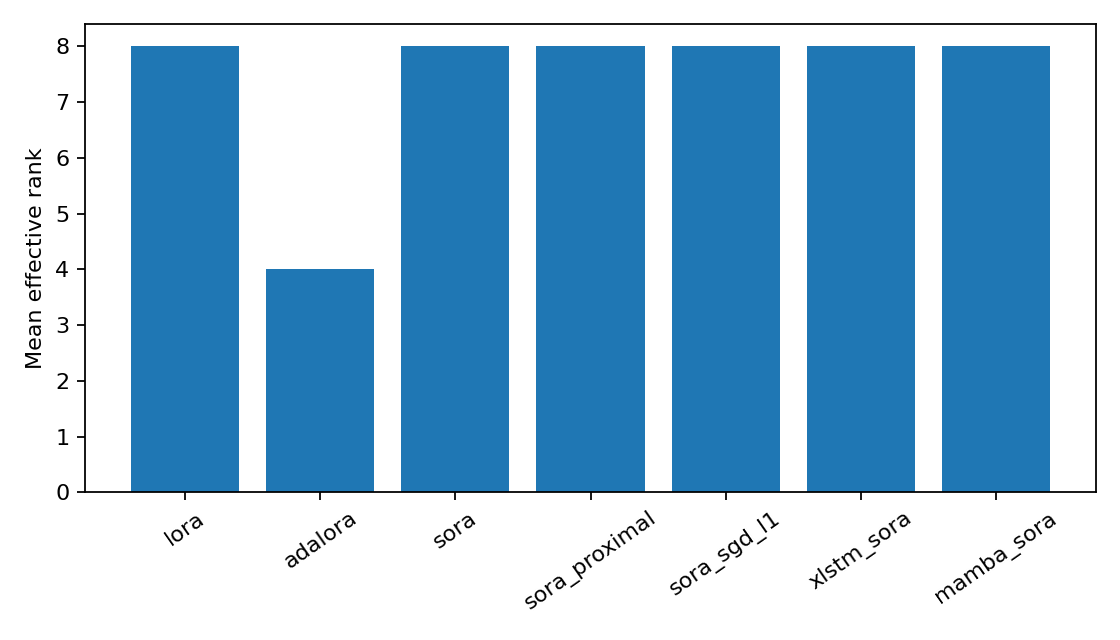
\includegraphics[width=0.7\linewidth]{../../results/sparsity_deberta_long/effective_rank.png}
\caption{Effective rank after adapter training. AdaLoRA prunes to the configured lower rank.}
\label{fig:effective-rank}
\end{figure}

The important point here is that the longer run gave me the real CoLA numbers I wanted. SoRA was the strongest result in the final table, AdaLoRA did exactly what it was supposed to do by reducing effective rank, and the proximal-vs-SGD comparison stayed in the same metric pipeline.

\subsection{xLSTM and Mamba Extension}
I reused the same adapter idea on two non-Transformer backbones because the assignment asked me to check whether sparse adaptation transfers beyond Transformers.

In \texttt{sparsity/toy\_models.py}, the xLSTM path attaches adapters to the input projection, recurrent projection, and classifier. The Mamba-style path attaches adapters to the input, delta, state-input, state-readout, output, and classifier projections. In the final WSL environment, those runs use the installed \texttt{xlstm} and \texttt{mamba\_ssm} packages when available, while the fallback PyTorch paths stay around for CPU-only tests.

The reason the adapter placement changes is simple: these backbones do not expose the same projection structure as a Transformer. If I reused Transformer insertion points blindly, the adaptation would miss the linear maps that actually control state flow and token mixing.

What I found here was that the transfer is structurally easy, but the performance is not especially strong without more tuning. That feels like a fair result to report honestly.

\subsection{Implementation Challenges}
Several practical issues came up while I was building the sparse side.

\subsubsection{Adapter Placement}
The first challenge was deciding where to insert adapters. The theory is simple, but the actual model structure matters a lot. I had to make sure the adapters were placed on meaningful projection layers rather than just anywhere that happened to be a linear layer.

\subsubsection{Freezing Parameters Correctly}
Another important issue was freezing the pretrained backbone correctly. If I accidentally let base weights update, then the comparison would no longer be parameter-efficient and the whole experiment would stop meaning what I wanted it to mean.

\subsubsection{Tracking Effective Rank}
Nominal rank is easy to state, but effective rank is a more honest measure of what the model is really using. That became especially important when comparing LoRA, AdaLoRA, and SoRA.

\subsection{Sparse Results Summary}
The Sparsity section taught me that the main question is not ``can I squeeze the model down?'' The real question is ``how much capacity can I remove before task performance starts to break?'' That is the tradeoff the assignment wanted me to see.

The attention experiment showed that faster variants can still be competitive if the goal is to reduce compute. The LoRA, AdaLoRA, and SoRA results showed the same kind of balance on the PEFT side: lower rank and fewer active parameters can work well, but they usually give up a little accuracy. The xLSTM and Mamba extension reminded me that the same idea does not transfer perfectly to every architecture, which is still a useful result.

The broader lesson from this section is that you should not judge a method only by its final accuracy. Effective rank, parameter count, and training behavior matter too, especially if the whole point of the project is to understand what the method is really doing in practice.

I also came away with a better appreciation for measurement discipline. Once the same training loop is reused everywhere, the tables stop being random numbers and start telling an actual story.

\section{How I Ran the Project}
The project is driven by the config files and sweep runners.

The main files I used are:
\begin{itemize}[leftmargin=*]
  \item \texttt{configs/core\_ml\_gpu.yaml}
  \item \texttt{configs/sparsity\_gpu.yaml}
  \item \texttt{configs/sparsity\_deberta\_long.yaml}
  \item \texttt{core\_ml/run\_suite.py}
  \item \texttt{sparsity/run\_suite.py}
\end{itemize}

The practical run order is:
\begin{enumerate}[leftmargin=*]
  \item prepare the environment and install dependencies
  \item download or confirm the GLUE CoLA data layout
  \item run the Core ML sweep
  \item run the bounded Sparsity sweep
  \item run the longer DeBERTa sweep for the final CoLA numbers
\end{enumerate}

The result folders then collect the per-run JSON files, summary CSVs, and plots that I used to write the report.

\section{Conclusion}
This assignment tied together architecture changes and parameter-efficient fine-tuning under one controlled local setup.

The Core ML section let me compare attention, positional encodings, and convolution hybrids inside one modular Transformer stack. The Sparsity section let me compare LoRA, AdaLoRA, SoRA, and the optimization behavior of sparse gates, and then check whether the same sparse-adapter idea could move to xLSTM and Mamba.

The biggest value of the project for me was not a single best score. It was seeing that the same framework could be reused across all of these comparisons with only the thing under study changing between runs.

That is really what the assignment was asking for, and that is what I tried to make clear in this report.

And honestly, the most useful thing for me was seeing the same idea survive across several different pieces of the stack. Once I had the pipeline set up properly, I could keep asking the same kind of question with different modules swapped in, which is exactly the kind of project flow I wanted from this assignment.

\end{document}
